\documentclass{article}
\usepackage[]{algorithm2e}
\usepackage{algpseudocode}
\usepackage{amsmath}
\usepackage{cleveref}
\usepackage{mathtools}
\usepackage{graphicx}
\usepackage{caption}
\usepackage{subcaption}

\newcommand{\cN}{{\mathcal{N}}}
\newcommand{\cAL}{{\mathcal{AL}}}
\newcommand{\cH}{{\mathcal{H}}}
\newcommand{\cGa}{{\text{Ga}}}
\newcommand{\cBe}{\text{Be}}

\newcommand{\cR}{{\mathcal{R}^\mathcal{D}}}
\newcommand{\cf}{{\mathbf{f}}}
\newcommand{\ce}{{\mathbf{e}}}
\newcommand{\cfs}{\mathbf{f_\star}}
\newcommand{\cx}{\mathbf{x}}
\newcommand{\cX}{\mathbf{X}}
\newcommand{\cxs}{\mathbf{x}_\star}
\newcommand{\ct}{{\mathbf{t}}}
\newcommand{\ceps}{{\mathbf{\epsilon}}}
\newcommand{\cI}{\mathbf{I}}
\newcommand{\cA}{\mathbf{A}}
%\newcommand{\cx}{{\mathbf{x}}}
\newcommand{\cB}{\mathbf{B}}
\newcommand{\cD}{\mathbf{D}}
\newcommand{\czero}{{\mathbf{0}}}
\newcommand{\cK}{{\mathbf{K}}}
\newcommand{\cSigma}{{\mathbf{\Sigma}}}
\newcommand{\cem}{{\mathbf{\m}}}
\newcommand{\cmu}{{\bm{\mu}}}
\newcommand{\ckappa}{{\bm{\kappa}}}
\newcommand{\ctheta}{\bm{\theta}}
\newcommand{\cexp}{{\text{exp}}}
\newcommand{\csI}{\sigma^2\cI}
\newcommand{\cts}{\cf}
\newcommand{\cData}{\mathcal{D}}
\newcommand{\cPhi}{\bm{\Phi}}
\newcommand{\Pzun}{p(z)}
\newcommand{\cpt}{\int_0^{\infty}\Pzun p(\cy|z)\,dz}
\newcommand{\cptb}{\int_0^{\infty}\Pzun~\cN(\cy| \czero,z\cK_{..})\,dz}
\newcommand{\cBess}{\mathcal{K}}
\newcommand{\cBessI}{\mathcal{I}}
\newcommand{\cint}{{\int_0^\infty}}
\newcommand{\cfKinvf}{\cf^T\cK^{-1}\cf}
\newcommand{\cGIG}{\text{GIG}}
\newcommand{\cpi}{\bm{\pi}}

\newcommand{\GIG}{{\mathbf{GIG}}}
\newcommand{\cEz}{\left\langle\frac{1}{z}\right\rangle_{q(z)}}
\newcommand{\cEzz}{\left\langle\frac{1}{z}\right\rangle}
\newcommand{\cEfKinvf}{\left\langle\cfKinvf\right\rangle_{q(\cf)}}
\newcommand{\czKsI}{\frac{1}{\cEzz_{q(z)}}\cK+\csI}
%angles paranthesis
\newcommand{\clangle}{\left\langle}
\newcommand{\crangle}{\right\rangle}
\newcommand{\chalf}[1]{\frac{1}{2#1}}
\newcommand{\css}{\sigma^2}
\newcommand{\clrbracket}[1]{\left(#1\right)}
\newcommand{\clrangle}[1]{\clangle#1\crangle}

\newcommand{\ctKinvt}{\cy^T\cK_{..}^{-1}\cy}
\newcommand{\cp}{\tilde{p}}
\newcommand{\ca}{\tilde{\alpha}}
\newcommand{\cat}{\mathbf{a}}
\newcommand{\cbt}{\mathbf{b}}
\newcommand{\cb}{\tilde{\beta}}
\newcommand{\cabt}{\ca\cb}

\newcommand{\cU}{\mathbf{U}}
\newcommand{\czKcsI}{z \cK+\csI}
\newcommand{\cKx}{\cK_{\cx,\cx}}
\newcommand{\cKsx}{\cK_{\cx_\star,\cx}}
\newcommand{\cKss}{\cK_{\cx_\star,\cx_\star}}
\newcommand{\cv}{\mathbf{v}}
\newcommand{\cz}{\mathbf{z}}

\newcommand{\cS}{\mathbf{S}}
\newcommand{\cw}{\mathbf{w}}
\newcommand{\cy}{\mathbf{y}}
\newcommand{\calpha}{\bm{\alpha}}
\newcommand{\clambda}{\bm{\lambda}}
\newcommand{\cgamma}{\bm{\gamma}}
\newcommand{\ceta}{\bm{\eta}}
\newcommand{\cbeta}{\bm{\beta}}

\newcommand{\caexp}{\alpha(1-\alpha)}
\newcommand{\csum}{\sum_{i=1}^{N}}
\newcommand{\csumt}{\sum_{t=1}^{T}}
\newcommand{\csumn}{\sum_{n=1}^{N}}

\newcommand{\vmf}{\text{vMF}}
\newcommand{\ga}{\text{Ga}}

\newcommand{\cfig}[3]{
\begin{figure}[h]
\centering
\includegraphics[]{#1}
\caption{#2}
\label{fig:{#3}}
\end{figure}
}

%For Dirichlet process
\newcommand{\cV}{\bigcup_{i=1}^{\infty}v_i}

%Didis commands
\newcommand{\ie}{{\sl i.e.}}
\newcommand{\eg}{{\sl e.g.}}
\newcommand{\etc}{{\sl etc.}}
\newcommand{\etal}{{\sl et al.}}

\newcommand{\cVprod}{\bigcup_{i=1}^{\infty}V_i}
\newcommand{\cVV}{\mathbf{V}}

\newcommand{\norm}[1]{\left\lVert#1\right\rVert}

\DeclareMathOperator*{\argmin}{\arg\!\min}

\newcommand{\cone}{\mathbf{1}}
\newcommand{\diag}{\text{diag}}
\newcommand{\Tr}{\text{Tr}}

\title{Reversible jump MCMC}
\date{}
\begin{document}
\maketitle




Reversible jump MCMC is a Bayesian algorithm to infer the number of components/ clusters from a set of data. For this illustration we shall consider a two component model at most.

The difficulty lies in considering the posterior given different number of components.

\section{Model}
The likelihoods can be represented as:
\begin{align}
p(y_i|\lambda_{d\cdot},k=state,z_{di})=&\prod_{j=1}^{d} (\lambda_{dj}\exp(-\lambda_{dj}y_i))^{1(z_{di}=j)}
\end{align}
where $d$ is the current dimensionality of the model. The priors on the latent variables are:
\begin{align}
p(\lambda_{dj})\propto & \frac{1}{\lambda_{dj}}\qquad \lambda_{dj}\in[a,b]\\
p(z_{di}=j)=&\pi_{dj}\\
p(\pi_{dj}) = & \text{Dir}(\alpha)\\
p(d=k)= & 1/K
\end{align}
$z_{di}$ is an indicator variable which chooses the relevant $\lambda_{dj}$ for the $i$-th observation. $K$ is the number of models that are being considered with differing dimensionality. $p(d=k)= 1/K$ implies that each model is equally probable. The limits on $\lambda_{dj}$ are such that $a=\min(1/y_i)$ and $b=\max(1/y_i)$ for all $j,k$. This is due to the fact that the mean of an exponential distribution is $1/\lambda$. Hence, it is a valid assumption that the mean of $1/y_i$ lies between $a$ and $b$. $\alpha$ is chosen to be $1$ such that it portrays a uniform distribution over $[0,1]$.

Marginalising out $z_{dj}$ we obtain:
\begin{align}
p(y_i|\lambda_{d\cdot},d=k)= \sum_{j=1}^{k}\pi_{kj}\lambda_{kj}\exp(-\lambda_{kj}y_i)
\label{eq:lik}
\end{align}

\section{Jumping dimensions}
We need to consider a Metropolis-Hastings (MH) step to consider going from one component to two components. The MH step in general is as follows:
\begin{align}
\alpha = & \frac{p\clrbracket{\theta_{d(t+1)}|\cy}}{p\clrbracket{\theta_{d(t)}|\cy}}\frac{q\clrbracket{\theta_{d(t)}|\theta_{d(t+1)}}}{q\clrbracket{\theta_{d(t+1)}|\theta_{d(t)}}}\\
A = & \text{min}\left(1,\alpha\right)
\end{align}
where $d(t)$ is the dimensionality at time $t$ and $\theta_{d(t)}=\{\lambda_{d(t)\cdot},\pi_{d(t)\cdot}\}$. The proportion $\frac{p\clrbracket{\theta_{d(t+1)}|\cy}}{p\clrbracket{\theta_{d(t)}|\cy}}$ can be rewritten as,
\begin{align}
\frac{p\clrbracket{\theta_{d(t+1)},\cy}}{p\clrbracket{\theta_{d(t)},\cy}}
\end{align}
since $p(\cy)$ is independent of dimensionality and, can be evaluated using equation \ref{eq:lik} as,
\begin{align}
\frac{\clrbracket{\prod_{i=1}^{N}\sum_{j=1}^{d(t+1)}\pi_{kj}\lambda_{kj}\exp(-\lambda_{kj}y_i)}\prod_{j=1}^{d(t+1)}p(\lambda_{d(t+1)j})p(\pi_{d(t+1)})p(d=d(t+1))}{\clrbracket{\prod_{i=1}^{N}\sum_{j=1}^{d(t)}\pi_{kj}\lambda_{kj}\exp(-\lambda_{kj}y_i)}\prod_{j=1}^{d(t)}p(\lambda_{d(t)j})p(\pi_{d(t)})p(d=d(t))}
\end{align}
The proposal distributions are as follows (for $d(t)=d(t+1)-1$):
\begin{align}
q\clrbracket{\theta_{d(t)}|\theta_{d(t+1)}}=q(d(t)|d(t+1))q(idx)q(\lambda_{d(t)}|\lambda_{d(t+1)},idx)q(\pi_{d(t)}|\pi_{d(t+1)},idx)
\end{align}

\subsection{Jumping from 1 dim to 2}
In this case let the parameters $\theta_2=\{\lambda_{12},\lambda_{22},k,\pi\}$ and $\theta_1=\{\lambda_{11},k\}$. As we can let the proposal distribution be anything, we let $q(\theta_1\to\theta_2)$ as follows:
\begin{align}
q(\lambda_{j2},\pi,k=2|k=1,\lambda_{11})=q(\lambda_{j2}|k=2,\lambda_{11})q(\pi|k=2)q(k=2|k=1)
\end{align}
We let the \textbf{proposal} $q(k=2\vert k=1)=1$. We also have the following dimensional jump:
\begin{align}
\mu_1,\mu_2\sim & \,U(0,1)\\
\lambda_{12}=&\lambda_{11}\frac{\mu_1}{1-\mu_1}
\label{eq:lambda_12}\\
\lambda_{22}=&\lambda_{11}\frac{1-\mu_1}{\mu_1}
\label{eq:lambda_22}\\
\pi=&\mu_2
\end{align} 

Thus, in order to find the distribution $q(\lambda_{j2}\vert k=2,\lambda_{11})$ we use the change of variable identity that $q(\lambda_{j2}\vert k=2,\lambda_{11})=q(\mu_1)\vert J\vert$ where, $J$ is the Jacobian $\frac{\partial(\lambda_{11},\mu_1)}{\partial(\lambda_{12},\lambda_{22})}$. Using \crefrange{eq:lambda_12}{eq:lambda_22} the inverse Jacobian is found to be:
\begin{align}
J^{-1}=\begin{bmatrix}
\frac{\mu_1}{1-\mu_1} & \lambda_{11}\frac{1}{(1-\mu_1)^2}\\
\frac{1-\mu_1}{\mu_1} & -\lambda_{11}\frac{1}{\mu_1^2}
\end{bmatrix}
\end{align}
Hence the determinant is of the Jacobian determinant is found to be $\frac{\mu_1(1-\mu_1)}{2\lambda_{11}}$ while $q(\mu_1)=q(\mu_2)=1$ since they are sampled from standard uniform distributions. Also $q(\mu_2)=q(\pi\vert k=2)$.

Since we need the ratio of proposed states $ \frac{q(\theta_1^t|\theta_2^{t+1})}{q(\theta_2^{t+1}|\theta_1^{t})} $ we are also required to find $ q(\lambda_{11},k=1\vert\lambda_{2j},\pi,k=2) = q(\lambda_{11}\vert\lambda_{2j},k=1) q(k=1 \vert k=2) $. We again take $ q(k=1\vert k=2)=1 $. $q(\lambda_{11}=\sqrt{\lambda_{12}\lambda_{22}})=1$, i.e. support at only point and zero at all other values of $\lambda_{11}$.
 
\subsection{Jumping from 2 to 1}
The MH step is conducted using the reciprocal of $\alpha$ in the equation above. Apart from the identity that $\lambda_{11}=\sqrt{\lambda_{12}\lambda_{22}}$ we also require the equation, $\mu_1=\frac{\lambda_{12}}{\lambda_{11}+\lambda_{12}}$ which can be derived from equation \ref{eq:lambda_12}. $\mu_2$ which is equivalent to $\pi$ can be taken to be the previous $\pi=\mu_2$ that was generated at state 2.

Note that this algorithm will not be sufficient to explore the posterior space. Consider $\lambda_{11}$ and note that currently it will only evaluate to one value, regardless of $\lambda_{12}, \lambda_{22}$. We employ a Gibbs sampler to efficiently explore each space separately.

\subsection{Gibbs Samplers}
\begin{align}
& p(\lambda_{11}|y,k=1) \propto \lambda_{11}^{N-1}\exp(-\lambda_{11}\sum_{i=1}^{N}y_i)\qquad \lambda_{11}\in[a,b]\\
& p(\lambda_{j2}|y,z,k=2) \propto \lambda_{j2}^{n_j-1}\exp(-\lambda_{j2}\sum_{i\in[j]}y_i)\qquad \lambda_{j2}\in[a,b]\\
& p(z_i=j|y,\lambda_{12},\lambda_{22}) \propto \lambda_{j2}\exp(-\lambda_{j2}y_i)\pi\\
& p(\pi) = Dir(\alpha+n_1,\alpha+n_2)
\end{align}

 \section{RJMCMC Algorithm}
 See Algorithm \ref{alg:post}.
\begin{algorithm}
%    \SetAlgoLined
    \KwData{$y_i$, iterations, $a$, $b$}
    \KwResult{Poseterior values of $\lambda_{11},\lambda_{2j}$ and state transitions.}
	Initialise $stateChain(1)=1$ and $\lambda_{1}Chain(1)\sim p(\lambda|a,b)$\\
    \For{$i =2:iterations$}{
    \eIf{state is 1}{
    $\lambda_{11}=\lambda_{1}Chain(last)$\\
    $\mu_1,\mu_2\sim  \,U(0,1)$\\
    $\lambda_{12}=\lambda_{11}\frac{\mu_1}{1-\mu_1}$\\
    $\lambda_{22}=\lambda_{11}\frac{1-\mu_1}{\mu_1}$\\
    $\pi=\mu_2$
    }{
	$\lambda_{12},\lambda_{22}=\lambda_{2}Chain(last)$\\
	$\lambda_{11} = \sqrt{\lambda_{12}\lambda_{22}}$\\
   	$\mu_1 = \frac{\lambda_{12}}{\lambda_{11}+\lambda_{12}}$
    }
    \vspace{-1cm}
    \begin{flalign*}
    & p(y|\lambda_{12},\lambda_{22},\pi,k=2) = \prod_{i=1}^N(\pi\lambda_{12}\exp(-\lambda_{12}y_i)+(1-\pi)\lambda_{22}\exp(-\lambda_{22}y_i))\\
    & p(\lambda_{12},\lambda_{22},\pi,k=2) = \frac{1}{C^2}\frac{1}{\lambda_{12}\lambda_{22}}\pi^{\alpha-1}(1-\pi)^{\alpha-1}\frac{1}{K}\\
    & p(y|\lambda_{11},k=1) = \lambda_{11}^N\exp(-\lambda_{11}\sum_{i=1}^{N}y_i)\\
    & p(\lambda_{11},k)=\frac{1}{C}\frac{1}{\lambda_{11}}\frac{1}{K}\\
    & \alpha_\star \coloneqq\left( \frac{p(y|\lambda_{12},\lambda_{22},\pi,k=2)p(\lambda_{12},\lambda_{22},\pi,k=2)}{p(y|\lambda_{11},k=1)p(\lambda_{11},k)}\right)\left(\frac{2\lambda_{11}}{\mu_1(1-\mu_1)}\frac{1}{q(\mu_1)q(\mu_2)}\right)
    \end{flalign*}    
    \If{state is 1}{
       	$\alpha_\star\coloneqq 1/\alpha_\star$
    }
    $A\coloneqq \min(1,\alpha_\star)$\\
    $u\sim U(0,1)$  \\
    \eIf{$A>u$}{
	    (Accept transition proposal)\\
	    \eIf{ state is 2}{
	    	$\lambda_1Chain.push(\lambda_{11})$\\
	    	$\lambda_1Chain.push(GibbsSampler1(y,a,b))$
	    }{
	    	$\lambda_2Chain.push(\lambda_{12},\lambda_{22})$
	    	$\lambda_2Chain.push(GibbsSampler2(y,\pi, \lambda_{12},\lambda_{22},\alpha,a,b))$
	    }
	    Switch states
	 }{\eIf{ state is 2}{
	     $\lambda_2Chain.push(\lambda_{12},\lambda_{22})$
	     	    	$\lambda_2Chain.push(GibbsSampler2(y,\pi, \lambda_{12},\lambda_{22},\alpha,a,b))$
	     }{
	     	$\lambda_1Chain.push(\lambda_{11})$\\
	     	    	$\lambda_1Chain.push(GibbsSampler1(y,a,b))$
	     }
	 }  
	 $stateChain.push([state state])$  
}
    \caption{}
    \label{alg:post}
    \end{algorithm}

\clearpage
\section{Results}
For this experiment data is generated as follows:
\begin{align*}
& \pi =  0.4 \\
& \lambda_{12},\lambda_{22} =  [2\quad 6] \\
& z_i \sim \pi^{1(z_i=1)}(1-\pi)^{1(z_i=2)}\qquad i=1,\cdots,N\\
& y_i \sim (p(y_i|\lambda_{12})^{1(z_i=1)}p(y_i|\lambda_{22})^{1(z_i=2)})\qquad i=1,\cdots,N
\end{align*}
where $p(y_i|\lambda_{j2})=\lambda_{j2}\exp(-\lambda_{j2}y_i)$.

The posterior $p(k=1|y)$ is calculated using the simulations and compared against the true posterior. The true posterior is,
\begin{align}
p(k=1|y)=&\frac{p(y|k=1)p(k=1)}{p(y|k=1)p(k=1)+p(y|k=2)p(k=2)}
\end{align}
since the prior $p(k=1)=p(k=2)$, it may be ignored from the above proportion.
\begin{align*}
p(y|k=1)=& \int \prod_{i=1}^{N}p(y_i|\lambda_{11},k=1)p(\lambda_{11}) d\lambda_{11}\\
p(y|k=2)=& \int \prod_{i=1}^{N}\left(\pi p(y_i|\lambda_{12},k=2)+(1-\pi)p(y_i|\lambda_{22},k=2)\right)p(\lambda_{12})p(\lambda_{22})p(\pi) d\lambda_{12}d\lambda_{22}d\pi
\end{align*}
In order to generate the exact posterior, we sample $10^6$ samples from the priors $p(\lambda_{11})$, $p(\lambda_{12})$, $p(\lambda_{22})$, $p(\pi)$. The posteriors are approximated as:
\begin{align}
p(y|k=1)\approx &\sum_{j=1}^{10^6}\prod_{i=1}^{N}p(y_i|\lambda_{11}^{(j)},k=1)\\
p(y|k=2)\approx & \sum_{j=1}^{10^6} \prod_{i=1}^{N}\left(\pi^{(j)} p(y_i|\lambda_{12}^{(j)},k=2)+(1-\pi^{(j)})p(y_i|\lambda_{22}^{(j)},k=2)\right)
\end{align}

The above `exact' posterior is compared against the simulated posterior. The relative number of state 1 from stateChain is the posterior probability from the simulated set.

\begin{table}[h]
\centering
\begin{tabular}{llll}
\hline
& \multicolumn{3}{c}{N}\\
\hline
& 50 & 100 & 200 \\
\hline
Exact & 0.63991 & 0.51736 & 0.00048488\\
Simulated & 0.64339 & 0.50834 & 0.00015789\\
\hline
\end{tabular}
\caption{Comparison of simulated and exact posterior of $p(k=1|y)$.}
\end{table}

The posterior $p(\lambda|y,k=1)$ and the posterior $p(\lambda|y,k=2)$ are plotted below in Figure \ref{fig:posteriors} for N=100 case.

\begin{figure}
\centering
\begin{subfigure}{0.3 \textwidth}
\centering
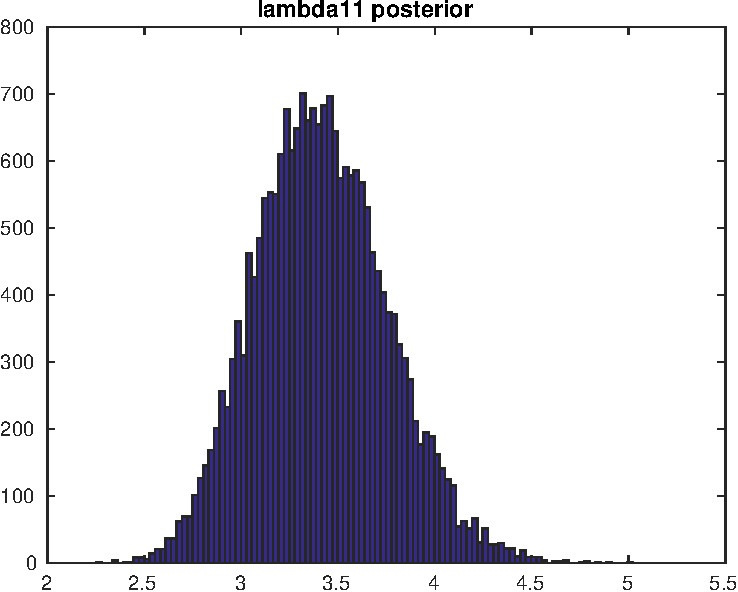
\includegraphics[height=1.5in]{lambda_11}
\caption{}
\end{subfigure}
\begin{subfigure}{0.3 \textwidth}
\centering
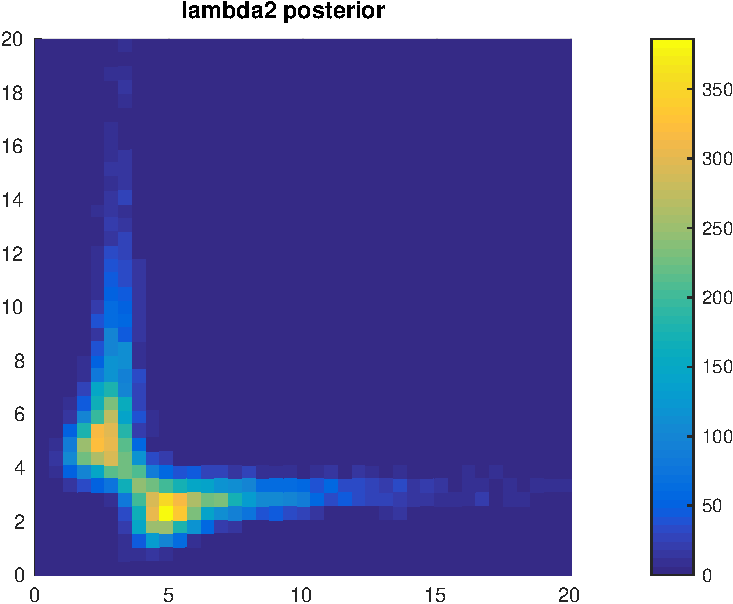
\includegraphics[height=1.5in]{lambda_22}
\caption{}
\end{subfigure}
\begin{subfigure}{0.3 \textwidth}
\centering
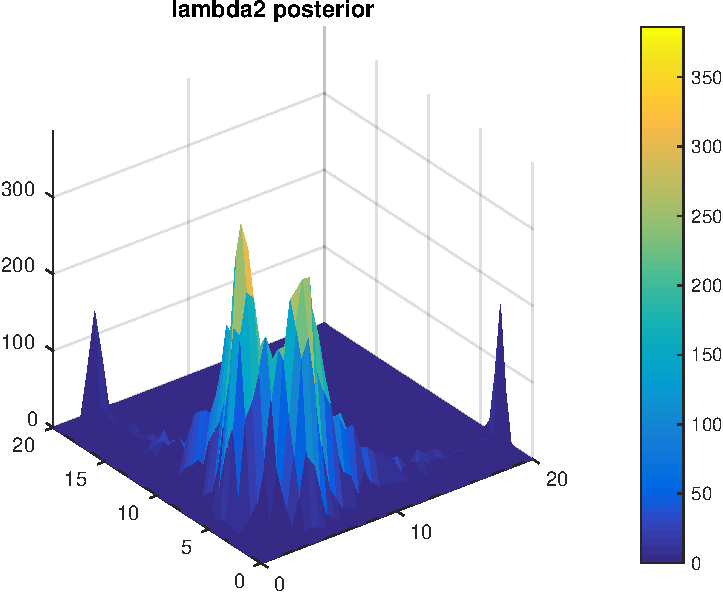
\includegraphics[height=1.5in]{lambda_22_3d}
\caption{}
\end{subfigure}
\caption{}
\label{fig:posteriors}
\end{figure}

\end{document}